\chapter{High Purity Germanium Detectors}
\label{chap:detectors}

\section{Introduction}
${}^{76}$Ge double-beta decays into ${}^{76}$Se, represented by the equation \ref{germanium_2nbb_eq}. It has several advantages as a source for $0\nu\beta\beta$ decay experiments. As a semiconductor, it can be made into detectors with excellent energy resolution, which is critical because energy is the only observable that is both necessary and sufficient for a discovery. Its Q value is $2.039$ MeV, which is above the energies of most gamma events. The crystal growth process for Germanium has purification stages that can greatly reduce internal backgrounds such as $^{238}$U and $^{232}$Th chain contaminants. Germanium is abundant in nature and can be easily enriched, allowing for large-scale experiments. Signal formation inside Germanium is well understood and enables precise topology-based discrimination between background and signal events through pulse shape discrimination (PSD) techniques. High-purity germanium (HPGe) detectors thus have a long history in nuclear physics and rare event searches.


\begin{equation}\label{germanium_2nbb_eq}
{}_{32}^{76}Ge \rightarrow {}_{34}^{76}Se + 2e^- + 2\bar{\nu}_e
\end{equation}

Figure ~\ref{past_ge_exp} shows a timeline of HPGe-based experiments. Over the years, research and development have resulted in experiments that continuously provide a larger bound on the half-life of the reaction while reducing the background. 

\begin{figure}[!htb]
\centering
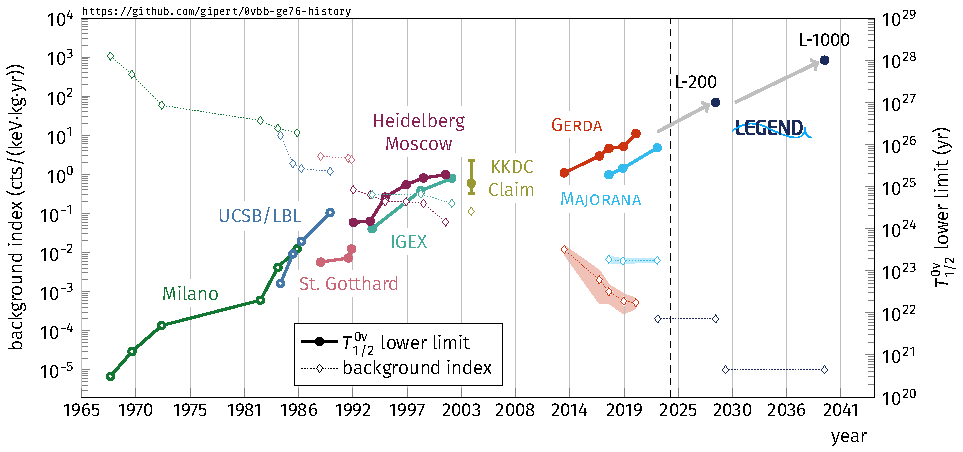
\includegraphics[trim=0.1cm 0 0.1cm 0,clip, width=0.99\linewidth]{ch2/figs/0nbb-ge76-history-future.pdf}
\caption{A plot showing a timeline of past and future HPGe {\onbb} decay experiments. The half-lives probed by them is shown along with their background index. Next generation experiments aim to continue improve half life limit while having the lowest background index. Picture credit: Luigi Pertoldi}
\label{past_ge_exp}
\end{figure}


\section{Signal formation in Germanium}
\subsection{Germanium properties}
The lattice structure of crystalline metals results in allowed energy bands for the electrons. The outermost bound state is termed the valence band, and the unbound state is termed the conduction band. The difference between the valence band and the minimal conduction band energy is called the band gap. Electrons of all lattice atoms can move freely in the conduction band. In metals, the band gap is nonexistent, with the valence and conduction bands overlapping, making metals very good conductors. In insulators, the band gap is large, making them poor electrical conductors.

In semiconductors, the band gap is intermediate ($2.96$ eV for Ge), which makes it possible to use semiconductor crystals as a radiation detector. Due to the ideal band gap, radiation excites multiple electrons to the conduction band, leaving behind a positively charged atom (hole). Both charge carriers can drift along the electric field and can be measured at a readout electrode. In reality, the holes do not drift. An electron from an adjacent atom fills the hole, another electron fills the new hole, and the process continues until the last hole is filled by the cathode. The process gives the illusion that the hole is drifting towards the negative terminal, and we will treat it as such. 

\subsection{P-type Point Contact Germanium Detectors}
A HPGe detector measures the total energy deposited by measuring the current induced by the drifting charge carriers on the readout electrodes. This is achieved by applying an external electric field to drift the charges towards the electrodes. There is still a steady leakage current as a result of the thermal excitation of the electrons. To reduce the leakage current, detectors are operated at low temperatures, but low electric fields make it difficult to efficiently detect radiation with just pure Germanium. Impurities are added to improve detector performance.

The impurities come in two forms: electron donors and receivers. The donors provide excess loosely bound electrons in the semiconductor, which is called the n-type, whereas the receivers increase the net number of holes, which is called the p-type. Impurities can be intentionally added to semiconductors to control the charge carriers and increase the conductivity by a process called doping. For example, doping Germanium with a group $15$ element such as Arsenic will make it n-type, since Arsenic has 5 valence electrons compared to four in Germanium. Similarly, doping Germanium with a group 13 element such as Aluminum (3 valence electrons) would make it p-type. \cite{knoll_2010}

During the manufacturing of an HPGe crystal, impurities are added to a molten bath, and the crystal is pulled via the Czochralski method. The concentration of impurities is not uniform throughout the crystal. In Germanium, this depends on the solubility ratio of the impurities in the solid and liquid phases, known as the segregation coefficient. A segregation coefficient close to $1$, such as that for Aluminum, will result in it being uniformly distributed in the crystal. For several n-type impurities such as Phosphorus and Oxygen, the segregation coefficient is less than $1$, and the impurities would prefer to be in a liquid state. As the crystal is pulled from its melt, the impurities with low segregation coefficients prefer the liquid phase and get concentrated in the bath. This will result in the tail having a higher impurity concentration. The net effect is an impurity gradient, which is important to consider while simulating signal formation inside the detector.

A diode is created when a p-type semiconductor is joined with an n-type semiconductor. The excess charges diffuse into each other, creating a region with no free charge carriers, called the depletion region. The process produces a net positive charge on the n side of the material and an equal-magnitude negative charge on the p side. This results in a potential difference across the material, termed the contact potential. If an external potential is applied opposite to the contact potential (positive potential on the p side, termed forward bias), there will be a free flow of current; however, if the external potential difference is applied opposite to the contact potential (positive potential on the n side, termed reverse bias), more charge carriers will diffuse, resulting in a larger depletion region and lower leakage current. This depletion region is ideal for detecting incident radiation, as the electrons ionized by the radiation are drifted by the bulk electric fields, creating a signal that is read out at the electrodes.

The depletion region can be inferred from the capacitance of the detector. The capacitance will continue to decrease until a certain potential, called the depletion voltage, is reached. The depletion voltage is where the biggest possible depletion region is achieved. Reducing the capacitance of HPGe detectors decreases the inherent noise in the readout circuit, thereby improving the energy resolution. This can be achieved by using a point-like central contact for the electrodes. In general, holes are less sensitive to charge trapping, and thus P-type detectors are preferred over N-type detectors for point-contact detector geometries.

\subsection{Shockley-Ramo Theorem}
Energy deposition in the detector will create charge clouds of electrons and holes. These charges induce an image charge on the point contact which is kept at zero potential. As these charge clouds drift under the electric field inside the detector, the image charges change, inducing a current at the point contact. The electrons and holes drift in opposite directions, resulting in a net negative induced signal on the read-out electrode. The Shockley–Ramo theorem gives the induced charge $Q(t)$ on an electrode caused by a moving charge $q$:

\begin{equation}\label{wp_eq}
Q(t)=q\Delta \phi_0(t)
\end{equation}
\noindent
The weighting potential $\phi_0(t)$ is the solution of the Laplace equation with the boundary conditions of $\phi_0=1$ for the readout electrode and $\phi_0=0$ for all other electrodes. Figure \ref{fig:wp_signal} left shows the calculated weighting potential inside a point contact detector used in {\Ltwo}. Note that the weighting potential is close to zero for most of the bulk. Thus, most energy depositions create charge clouds in the detector region with a low weighting potential. The holes travel to the p$^+$ point contact at the bottom and the electrons travel to the nearest n$^+$ region which surrounds the detector. Thus, holes undergo a larger change in the weighting potential than electrons since the point contact has a weighting potential of $1$. This bigger change means that the hole contribution dominates the signal. The holes encounter most of this potential difference in the region near the point contact, which results in a step-shaped signal shown by a sample waveform from a ${}^{76}$Ge detector in figure \ref{fig:wp_signal}.

  \begin{figure}[htb]
  \centering
   %[trim={left bottom right top},clip]
  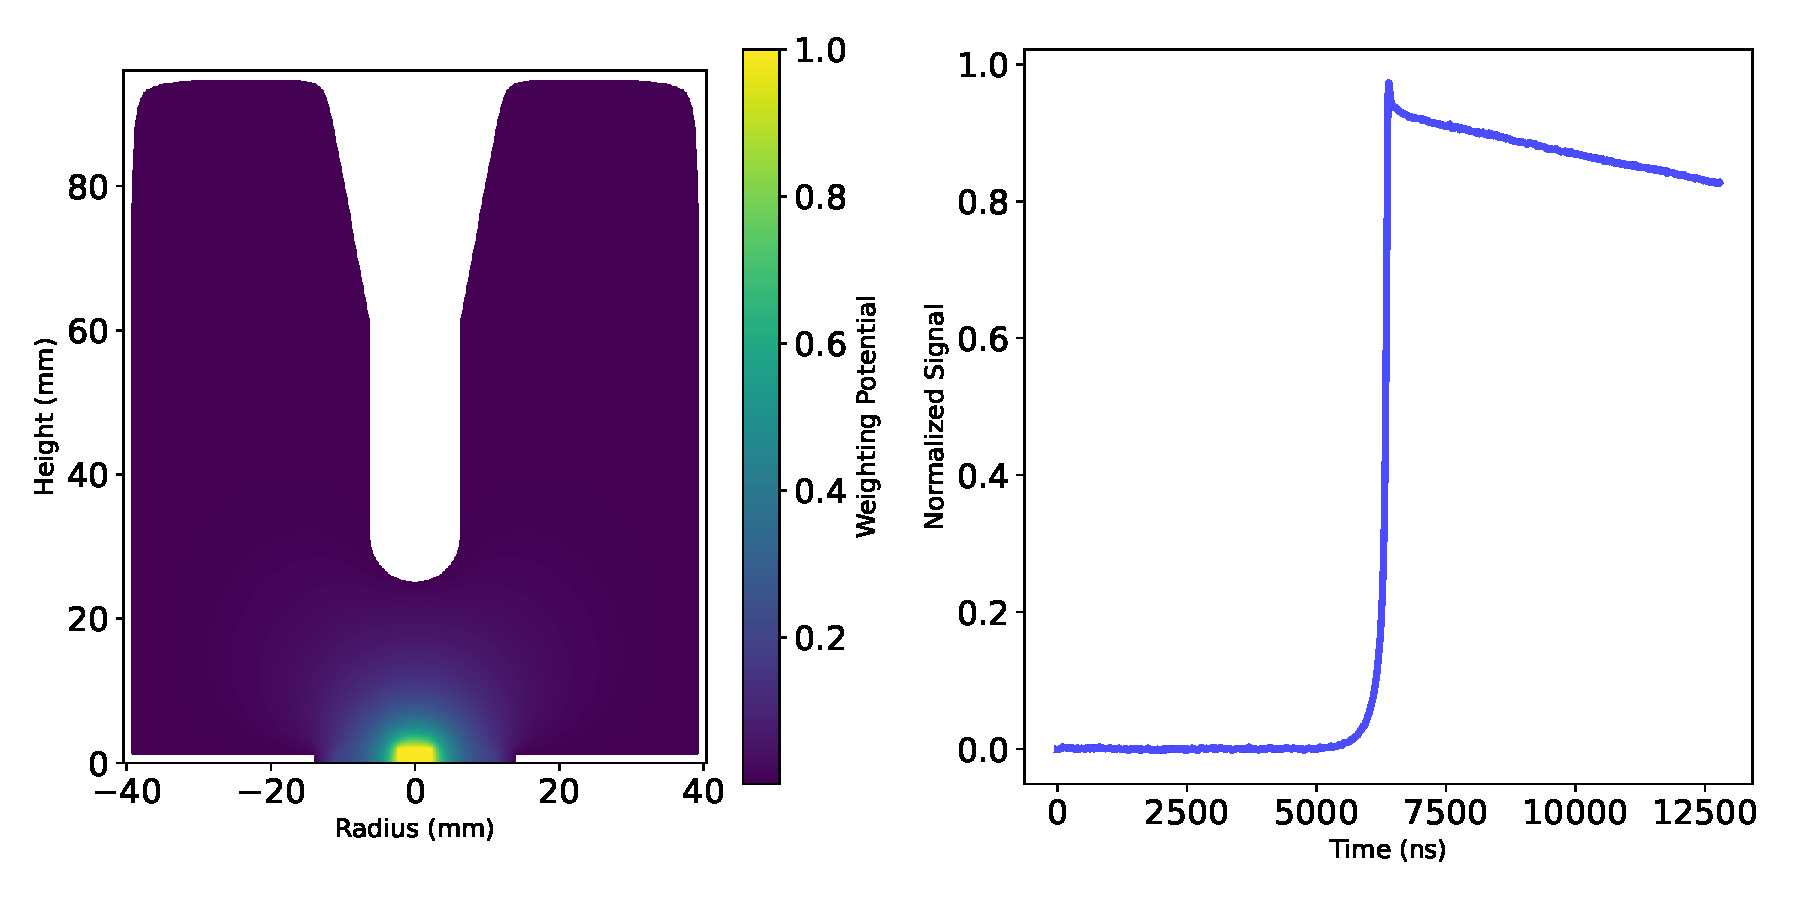
\includegraphics[trim=0 0.3cm 0 0,clip,width=\linewidth]{ch2/figs/wp_det.pdf}
  \caption{Left: Simulated weighting potential inside a LEGEND ICPC style point contact detector. Right: Collected signal from a detector showing sharp step shaped waveform.}
    \label{fig:wp_signal}
  \end{figure}

The pulse shape, along with a long drift time and a short collection time, provides an opportunity to veto multi-site events from gamma rays using analysis cuts. As the drift time varies with the path taken, multiple steps can often be identified in waveforms associated with multi-site events.

The {\MJ}, {\Gerda} and LEGEND collaborations are experiments with extensive experience in the research and development of HPGe detectors for {\onbb} searches.


\section{The {\MJD}}
The {\MJD} (MJD), located at the Sanford Underground Research Facility (SURF) in the USA, operated a $30$ kg array of enriched point-contact p-type (PPC) detectors developed by ORTEC. The detectors were divided between two vacuum-insulated cryostats housed within a low background shield and operated in a vacuum at liquid nitrogen (LN) temperature, as shown in figure \ref{fig:mjd}. 

MJD pioneered the development of underground electroformed copper (EFCu), where the purest commercially available Cu is obtained and electroformed underground to reduce contamination from cosmogenically produced $^{60}$Co. This also further reduced the concentration of natural contaminants $^{238}$ U and $^{232}$ Th by a factor of approximately 30 \cite{Abgrall:2016cct}. Another key innovation was the use of a low-mass front-end (LMFE) electronics board. The LMFE was designed to be highly radiopure and hence reduced the background close to the detector. It also reduced the noise in the signal, as the first stage of amplification occurred very close to the detector. With its ultra-clean procedures, underground electroformed Copper and advances in front-end electronics, MJD achieved the lowest energy resolution in any large scale {\onbb} decay experiment of $2.52$ keV ($0.12\%$) FWHM at $Q_{\beta\beta}$ when combining all detectors, and set a half-life limit $8.3 \times 10^{25}$ years ($90\%$ C.L.). {\MJD} had the second-lowest background index of $6.6 \times 10^{-3} \text{ cts/(keV kg yr)}$. \cite{Majorana_final}.

\begin{figure}
  \centering
  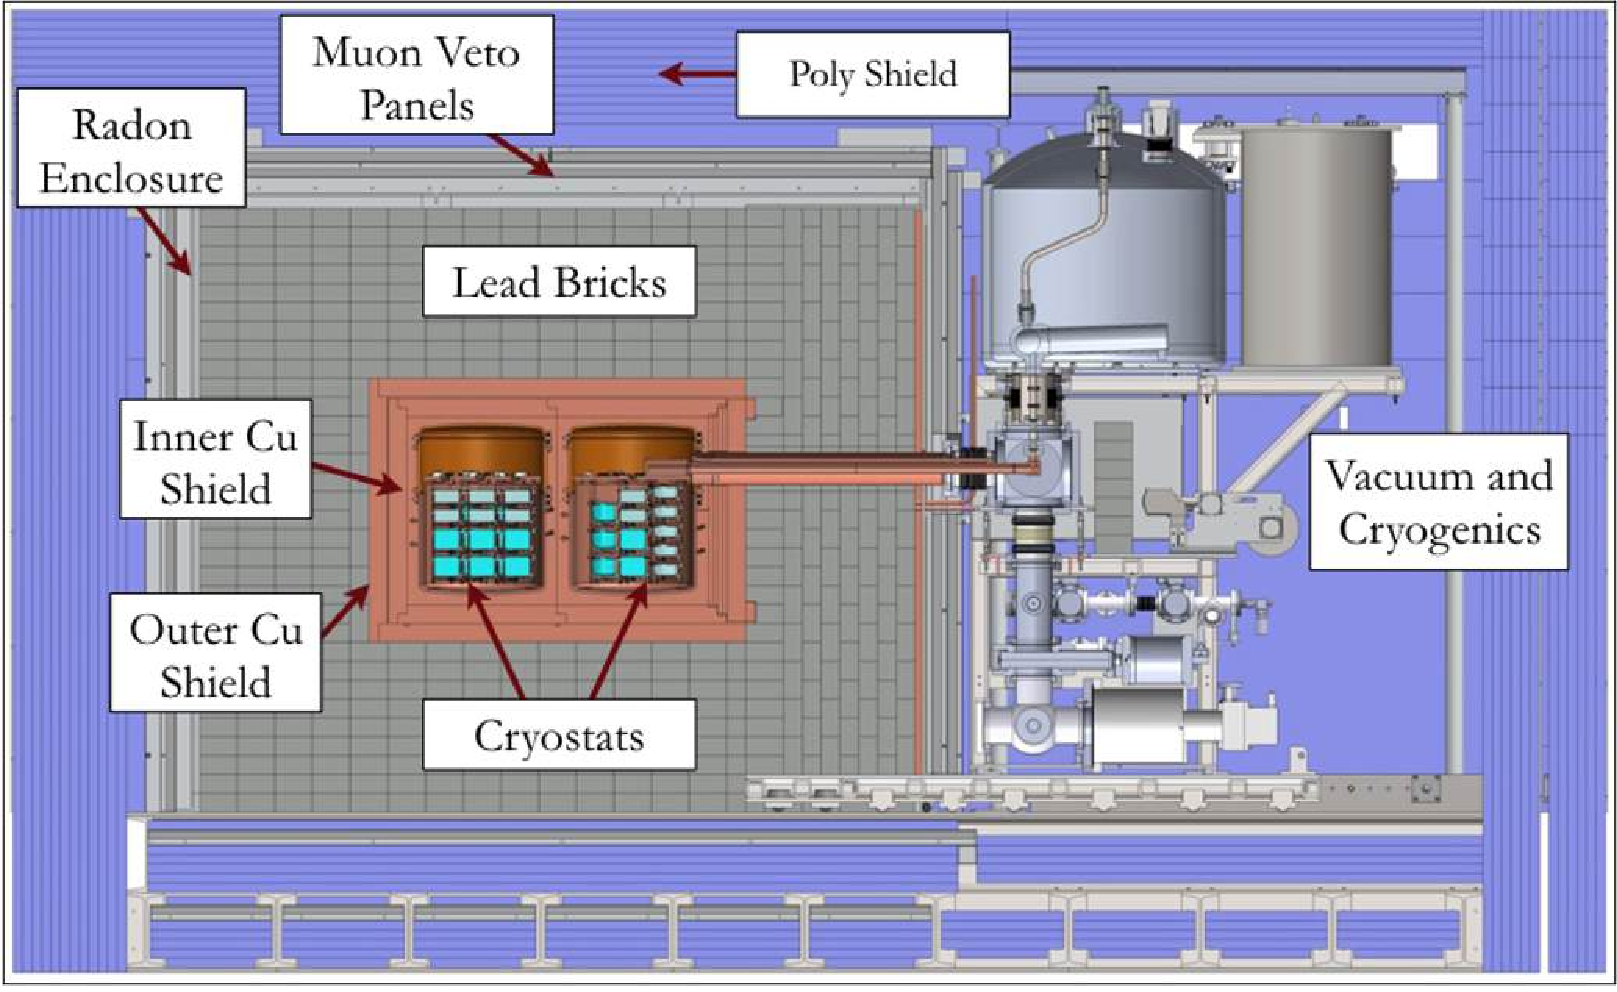
\includegraphics[height=0.34\columnwidth]{ch2/figs/mjd_setup.pdf}
  \qquad
  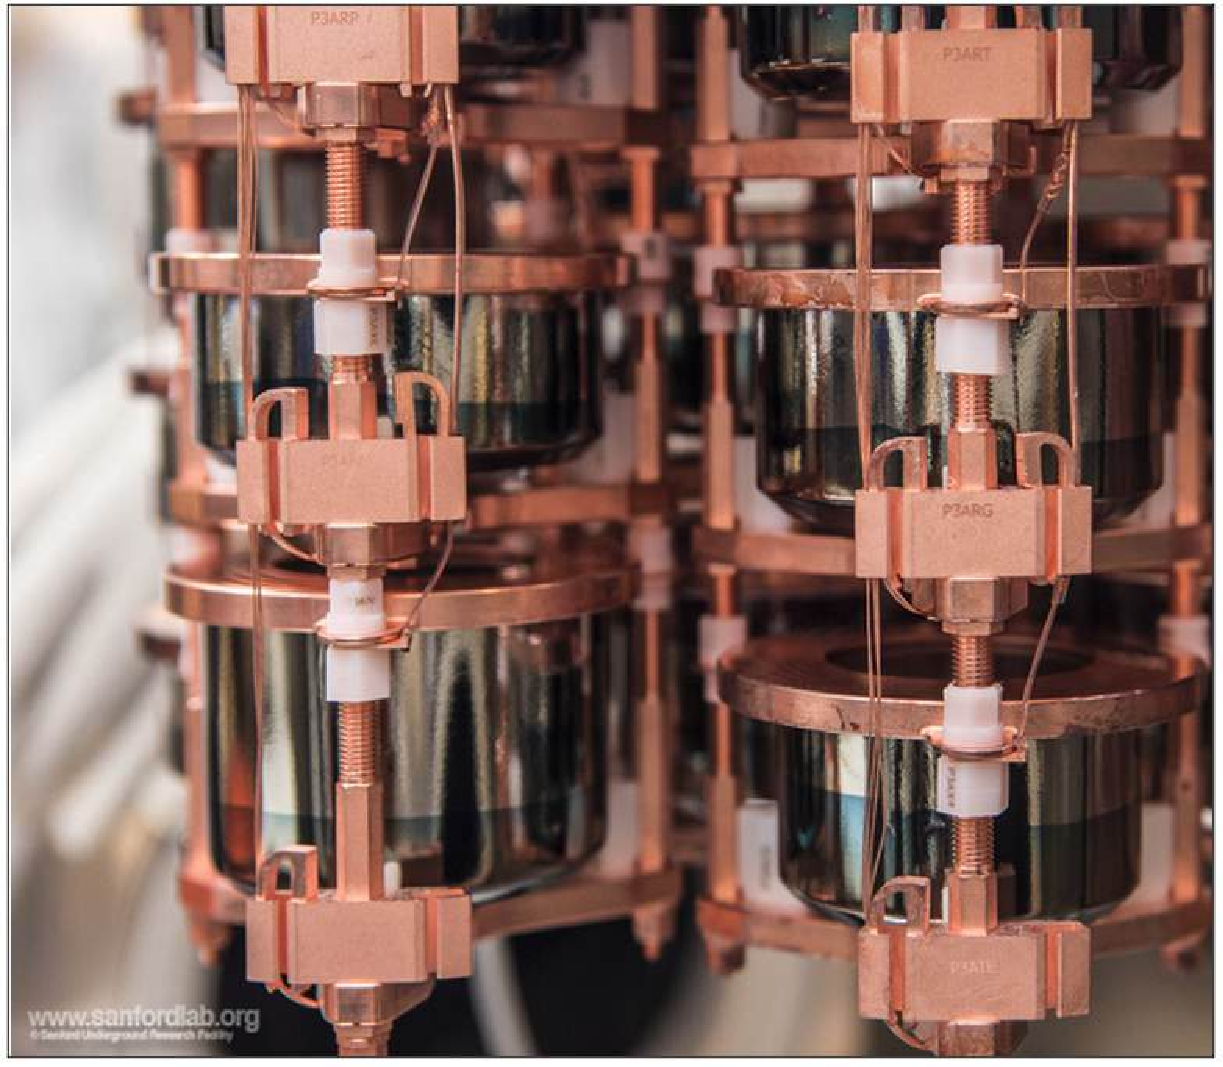
\includegraphics[height=0.34\columnwidth]{ch2/figs/mjd_ppc_array.pdf}
  \caption{The {\MJ} Demonstrator setup (left) and its Ge detector arrays (right).}
    \label{fig:mjd}
  \end{figure}
 
\section{The GERmanium Detector Array}
The GERmanium Detector Array ({\Gerda}) collaboration was another enriched Germanium detector-based experiment, located at the Laboratori Nazionali del Gran Sasso (LNGS) in Italy. {\Gerda} consisted of an array of $20$ kg of customized enriched versions of broad-energy Ge (BEGe) detectors and $15.6$ kg of enriched semicoaxial detectors developed by Mirion, as shown in figure \ref{ch2_fig_gerda_setup}. In its last year of data collection, {\Gerda} deployed an additional $9.6$ kg of the new p-type inverted coaxial point contact (ICPC) detectors to verify their technical maturity for future LEGEND experiments.

{\Gerda} took a unique approach to reduce background: operating the detectors in liquid Argon. The detector strings submerged in liquid Argon were surrounded by a shroud of wavelength-shifting fibers, and the entire LAr cryostat was surrounded by water that enabled a muon veto using Cherenkov radiation. The fibers converted Ar $128$ nm scintillation photons into green photons, which were observed using silicon photomultipliers (SiPM) attached to the ends of the fibers. This enabled a coincidence combining events detected in the Germanium detectors and the scintillation light read by SiPMs. The LAr veto allowed {\Gerda} to distinguish gamma backgrounds from {\onbb} signal candidate events with high efficiency, achieving a background rate of $5.2\times 10^{-4}$ cts/(keV kg yr) and reaching a half-life sensitivity greater than $10^{26}$ years \cite{GERDA_final}.

\begin{figure}
\centering
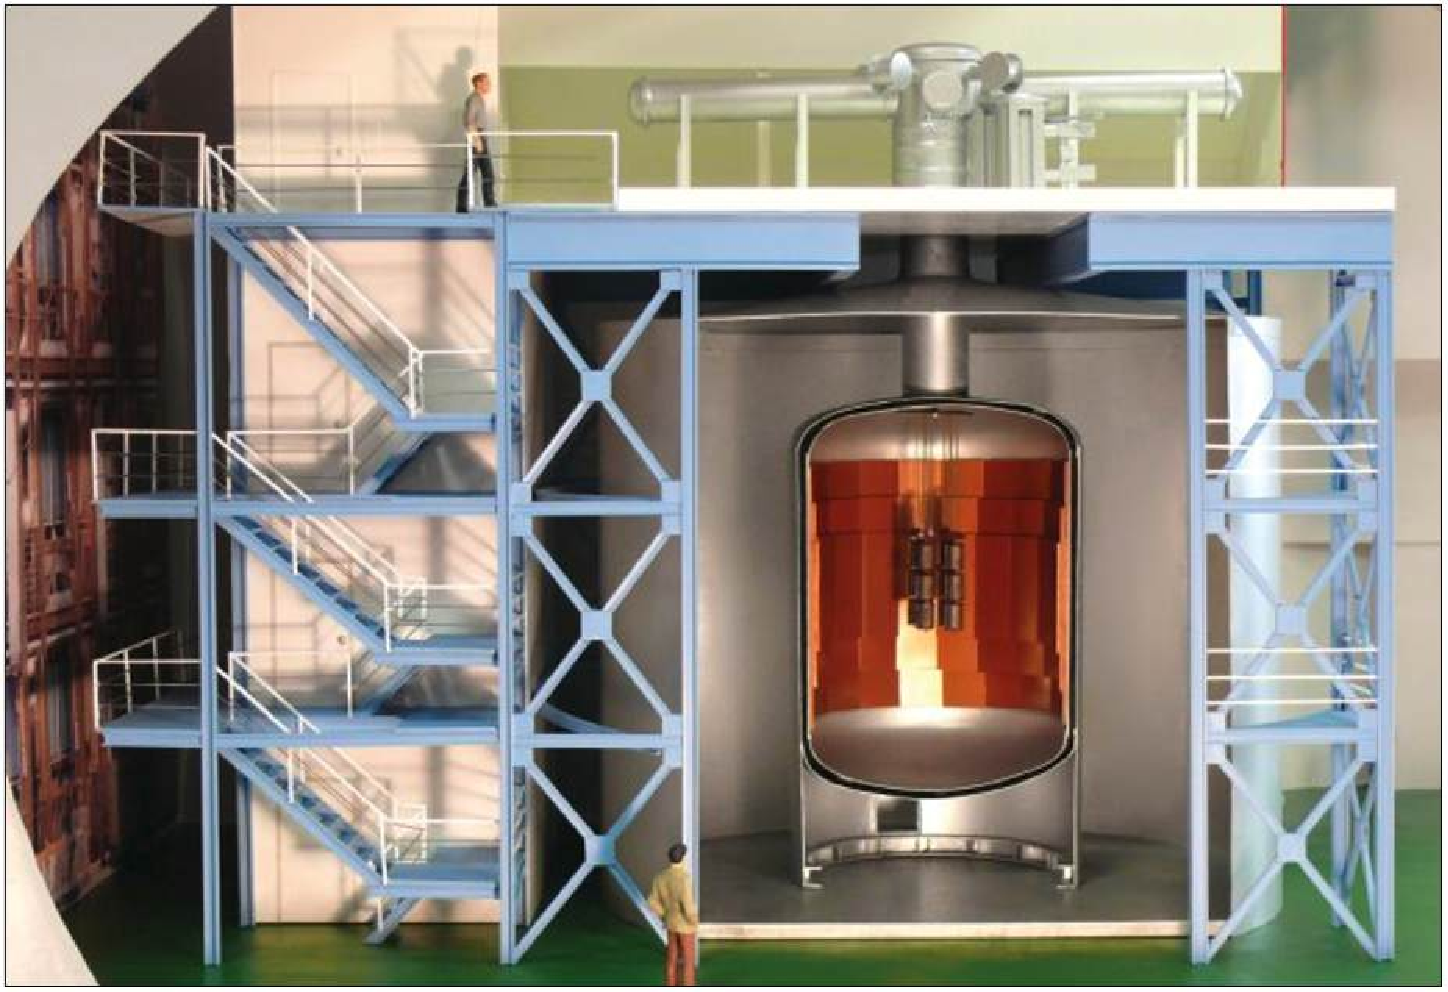
\includegraphics[height=0.385\columnwidth]{ch2/figs/gerda_setup.pdf}
\qquad
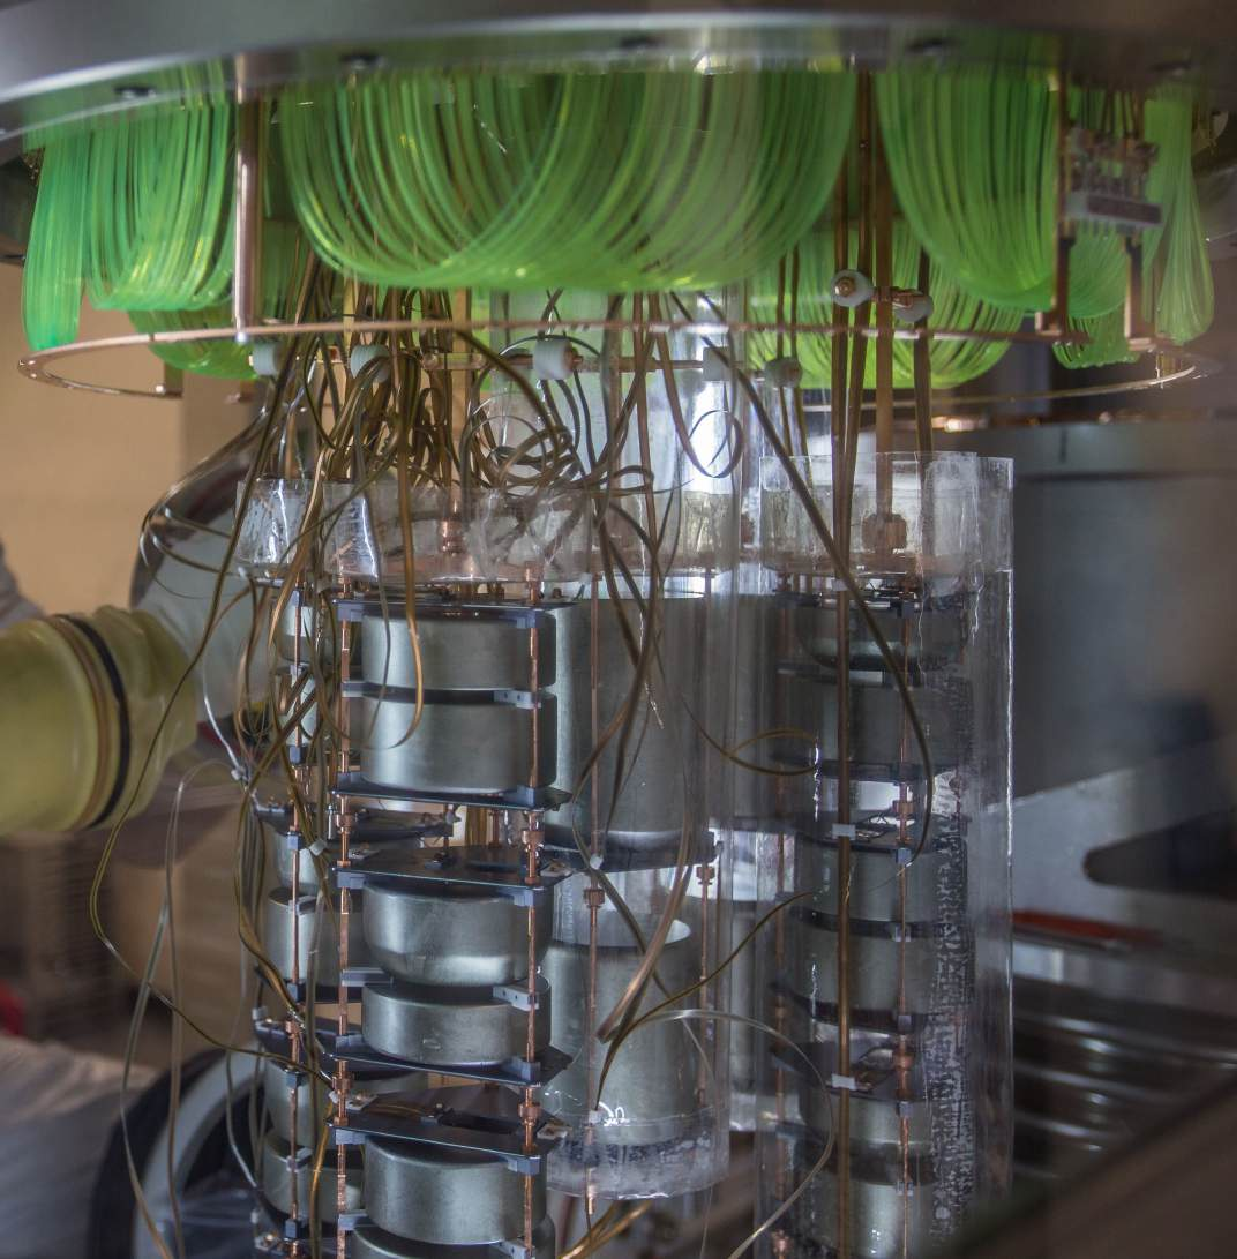
\includegraphics[height=0.385\columnwidth]{ch2/figs/gerdastrings.pdf}
\caption{{\Gerda} setup (left) with Ge detectors (right) arranged in vertical strings.}
\label{ch2_fig_gerda_setup}
\end{figure}
  
\section{The LEGEND experiment}
The Large Enriched Germanium Experiment for Neutrinoless $\beta\beta$ Decay (LEGEND) combines the best techniques and resources from {\Gerda} and MJD. In both previous experiments, the maximum mass of the detectors was constrained by the electrode geometry to $\sim1$ kg. Higher mass results in a lower surface-to-volume ratio, which reduces the per-channel background and decreases the number of channels needed, thus reducing per-kg background from cables, connectors, and detector mounts. A major innovation for LEGEND has been the development of p-type inverted-coaxial point contact (ICPC) detectors, which can be manufactured with masses of around $2-4$ kg \cite{COOPER201125}. LEGEND is taking a phased approach to a double-beta decay experimental program.

\subsection{LEGEND-200}
The first phase currently underway consists of $200$ kg of Germanium detectors housed in an upgrade of the {\Gerda} infrastructure at LNGS. In the first configuration, the MJD and {\Gerda} detectors constitute $55.8$ kg of the source mass, and the ICPC detectors $86.7$ kg. The setup is illustrated in figure \ref{fig:L200}. 

MJD achieved excellent energy resolution, primarily due to its low noise and low background electronics. The background model spectral fits indicated that the dominant background source in MJD was not from $^{208}$Tl sources close to the detectors. \cite{Buuck_thesis}. On the other hand, {\Gerda} achieved a lower background index with the help of its efficient LAr veto. The prominent features of its background model were the $^{210}$ Po on the surface of the Ge-detector p$^+$ electrode, $^{232}$Th and $^{238}$U decay chains, and $^{42}$Ar progeny. {\Gerda}'s background model fits of {\Gerda } suggest that the dominant background contributions \cite{GERDA_final} were from components close to the detector array.

{\Ltwo} inherits the best of both experiments. It uses MJD's low background materials and electronics to counter the background {\Gerda} observed closer to the detector and uses a LAr veto with improved scintillation light readout to reduce the distance-component backgrounds faced by MJD. The introduction of ICPC detectors also results in a lower surface-to-volume ratio, allowing for a reduction in net radioactive decays of alpha and beta particles near the surface. Higher-mass detectors also reduce the need for detector support materials and electronics that can be sources of background. 

\begin{figure}[!htb]
 \centering
 %[trim={left bottom right top},clip]
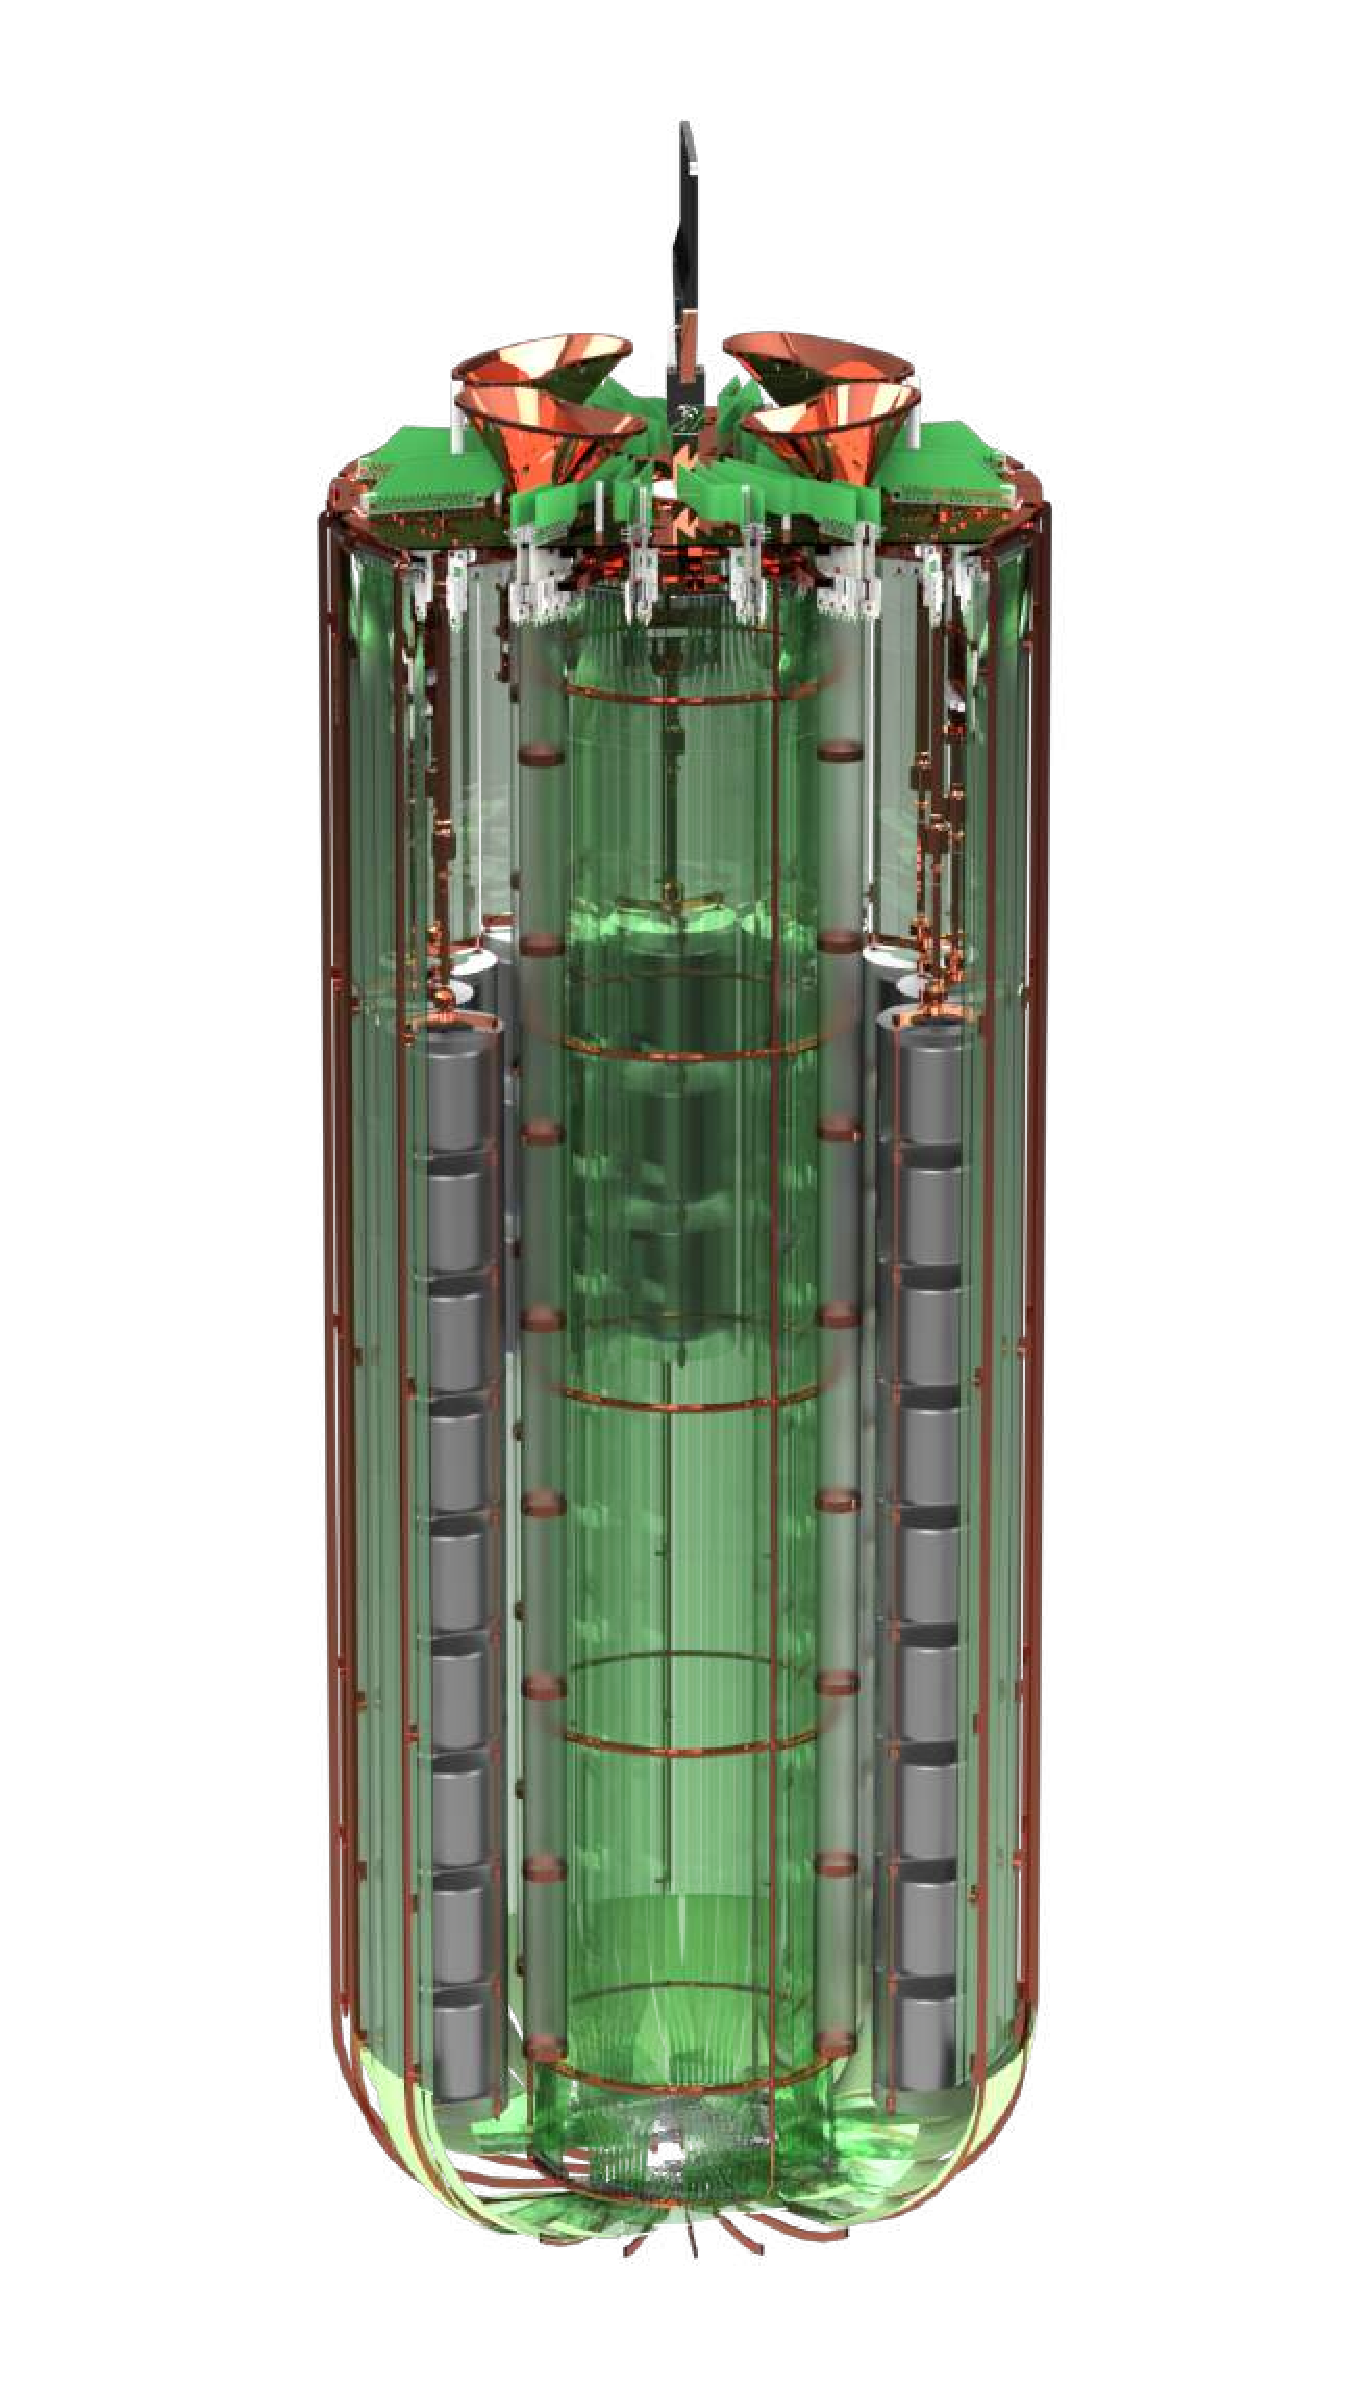
\includegraphics[trim=0 1cm 0 0,clip,height=0.4\linewidth]{ch2/figs/l200_strings.pdf}
\qquad
  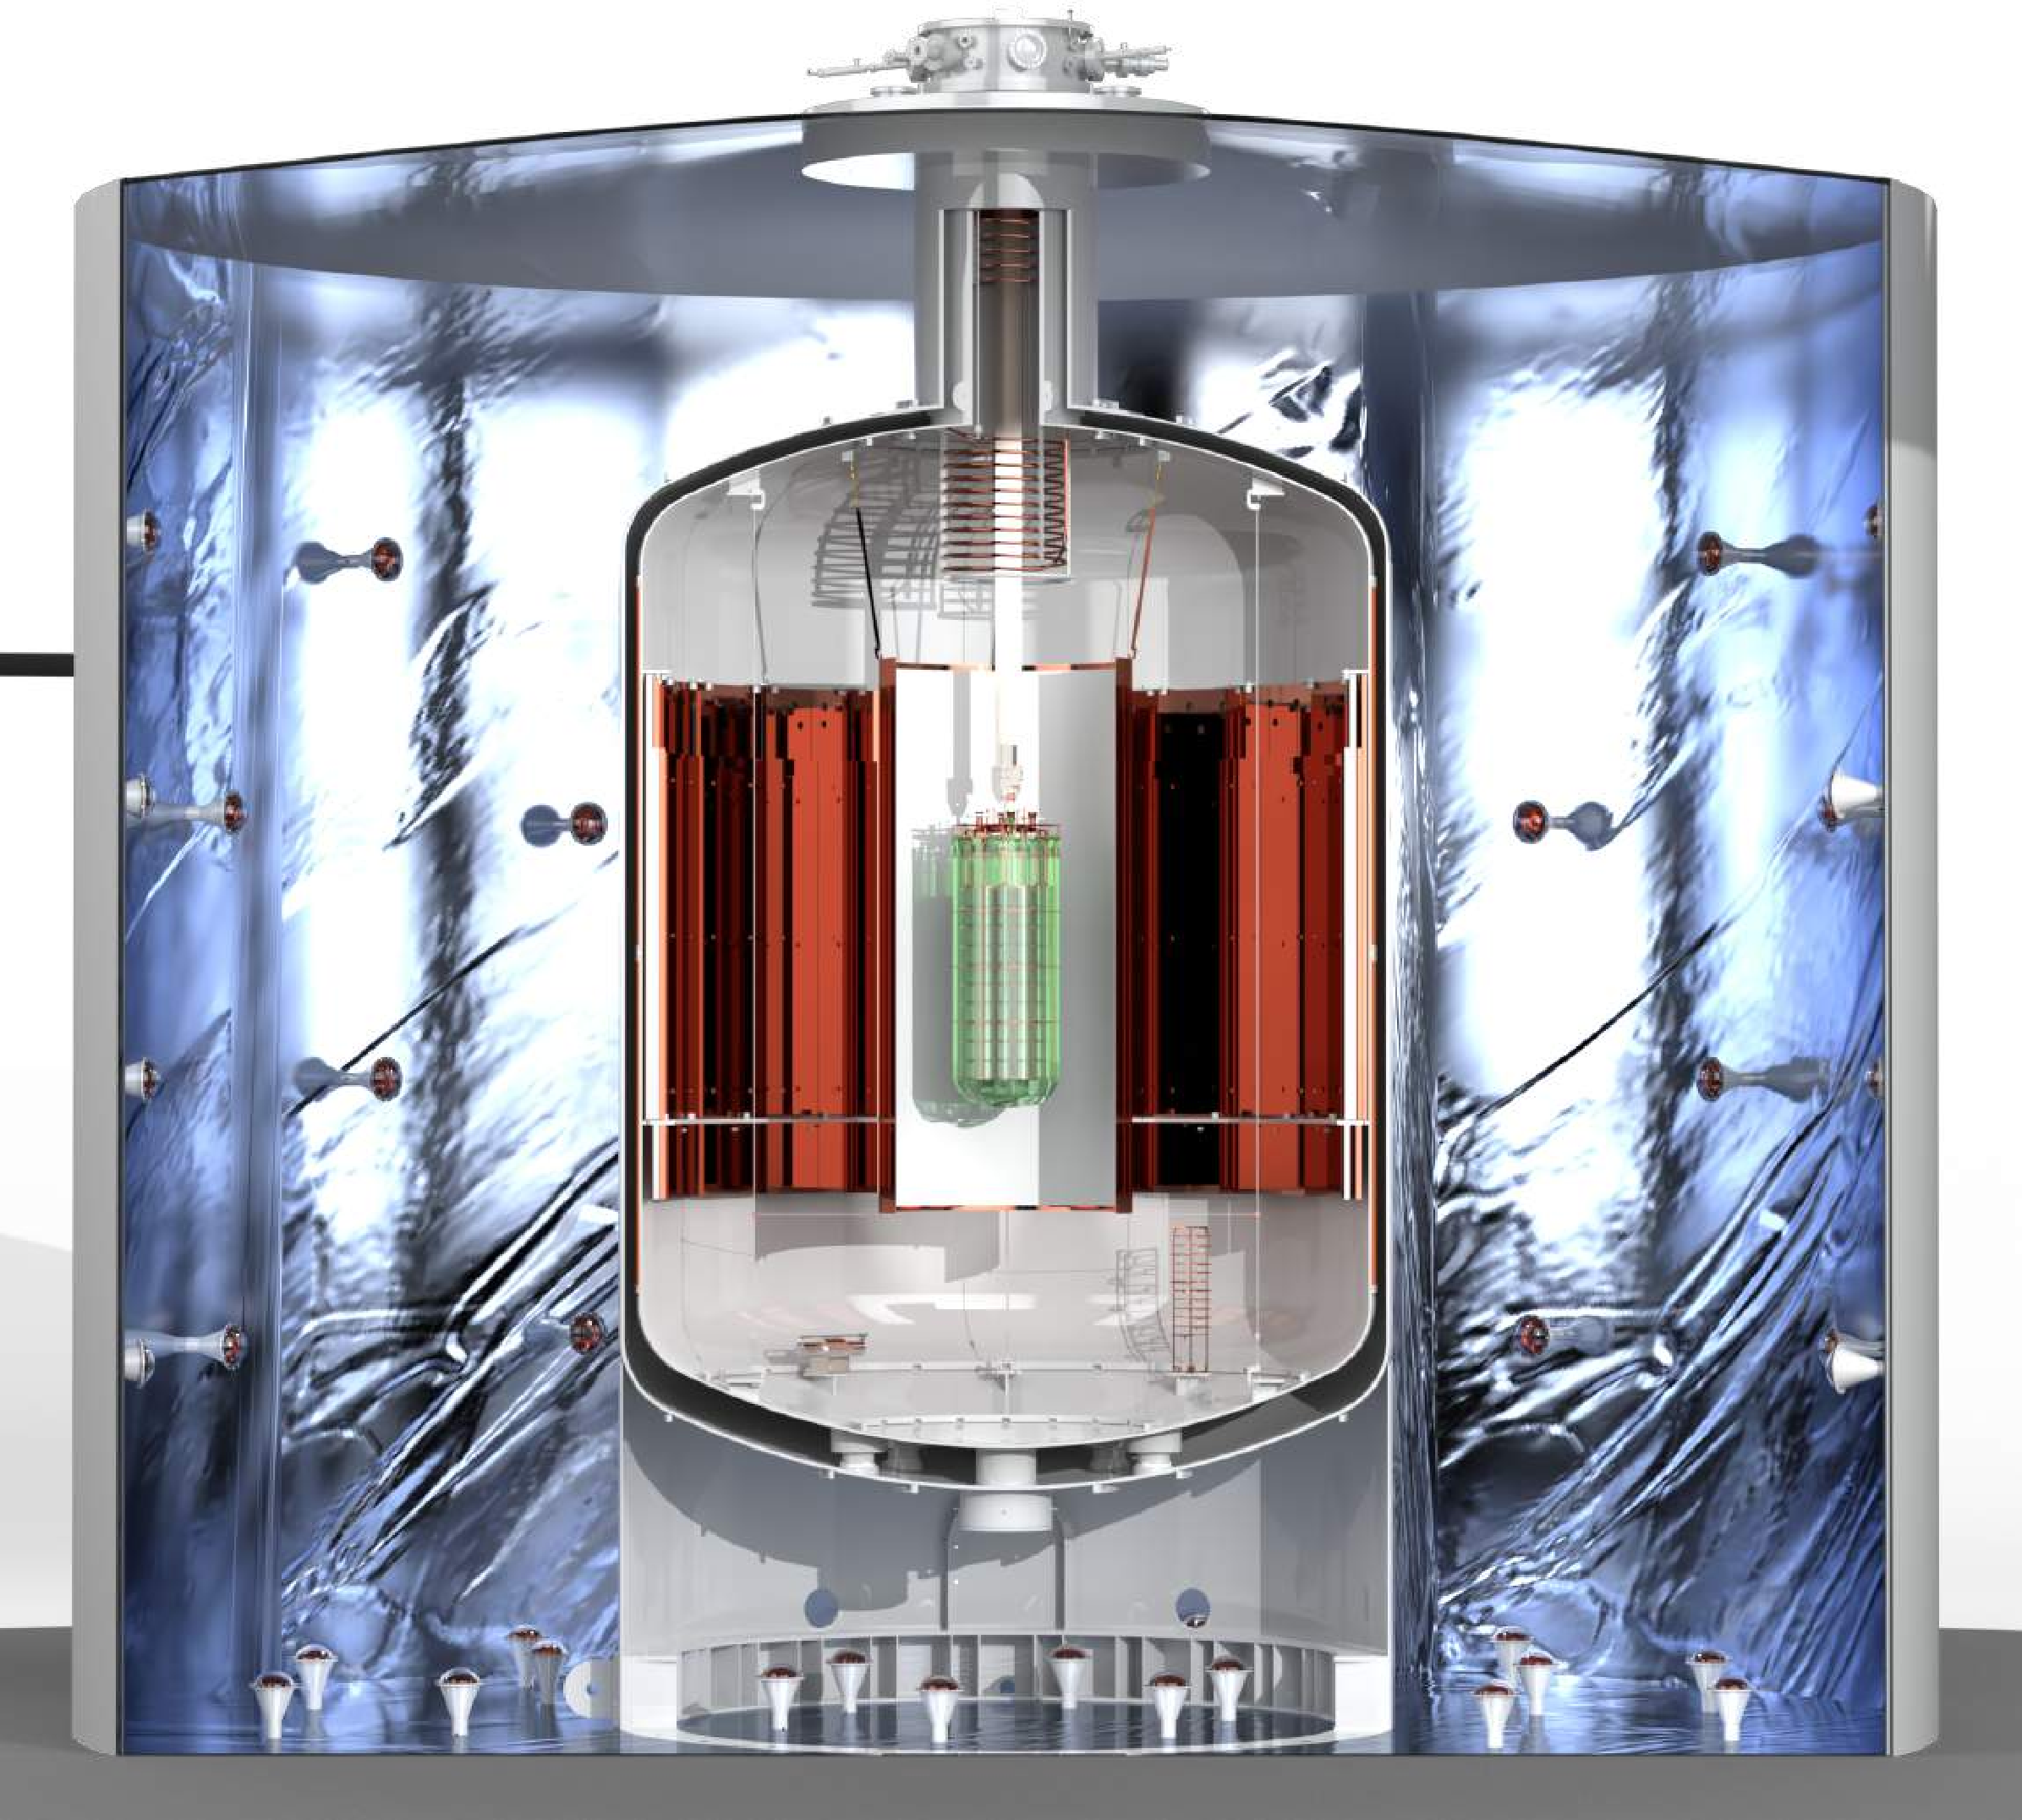
\includegraphics[height=0.4\linewidth]{ch2/figs/l200_fig.pdf}
 \caption{\label{fig:L200} Left: {\Ltwo} Ge detectors strings
 surrounded by wavelength-shifting fibers for LAr veto. Right: The L-200 design. The detector array is mounted in the center of the LAr cryostat. Muon veto is achieved by placing the cryostat in a water tank and detecting Cerenkov radiation with photo-multipliers. %\cite{l1000_pcdr} (Picture courtesy P. Krause).
}
\end{figure}

\begin{figure}[!htb]
  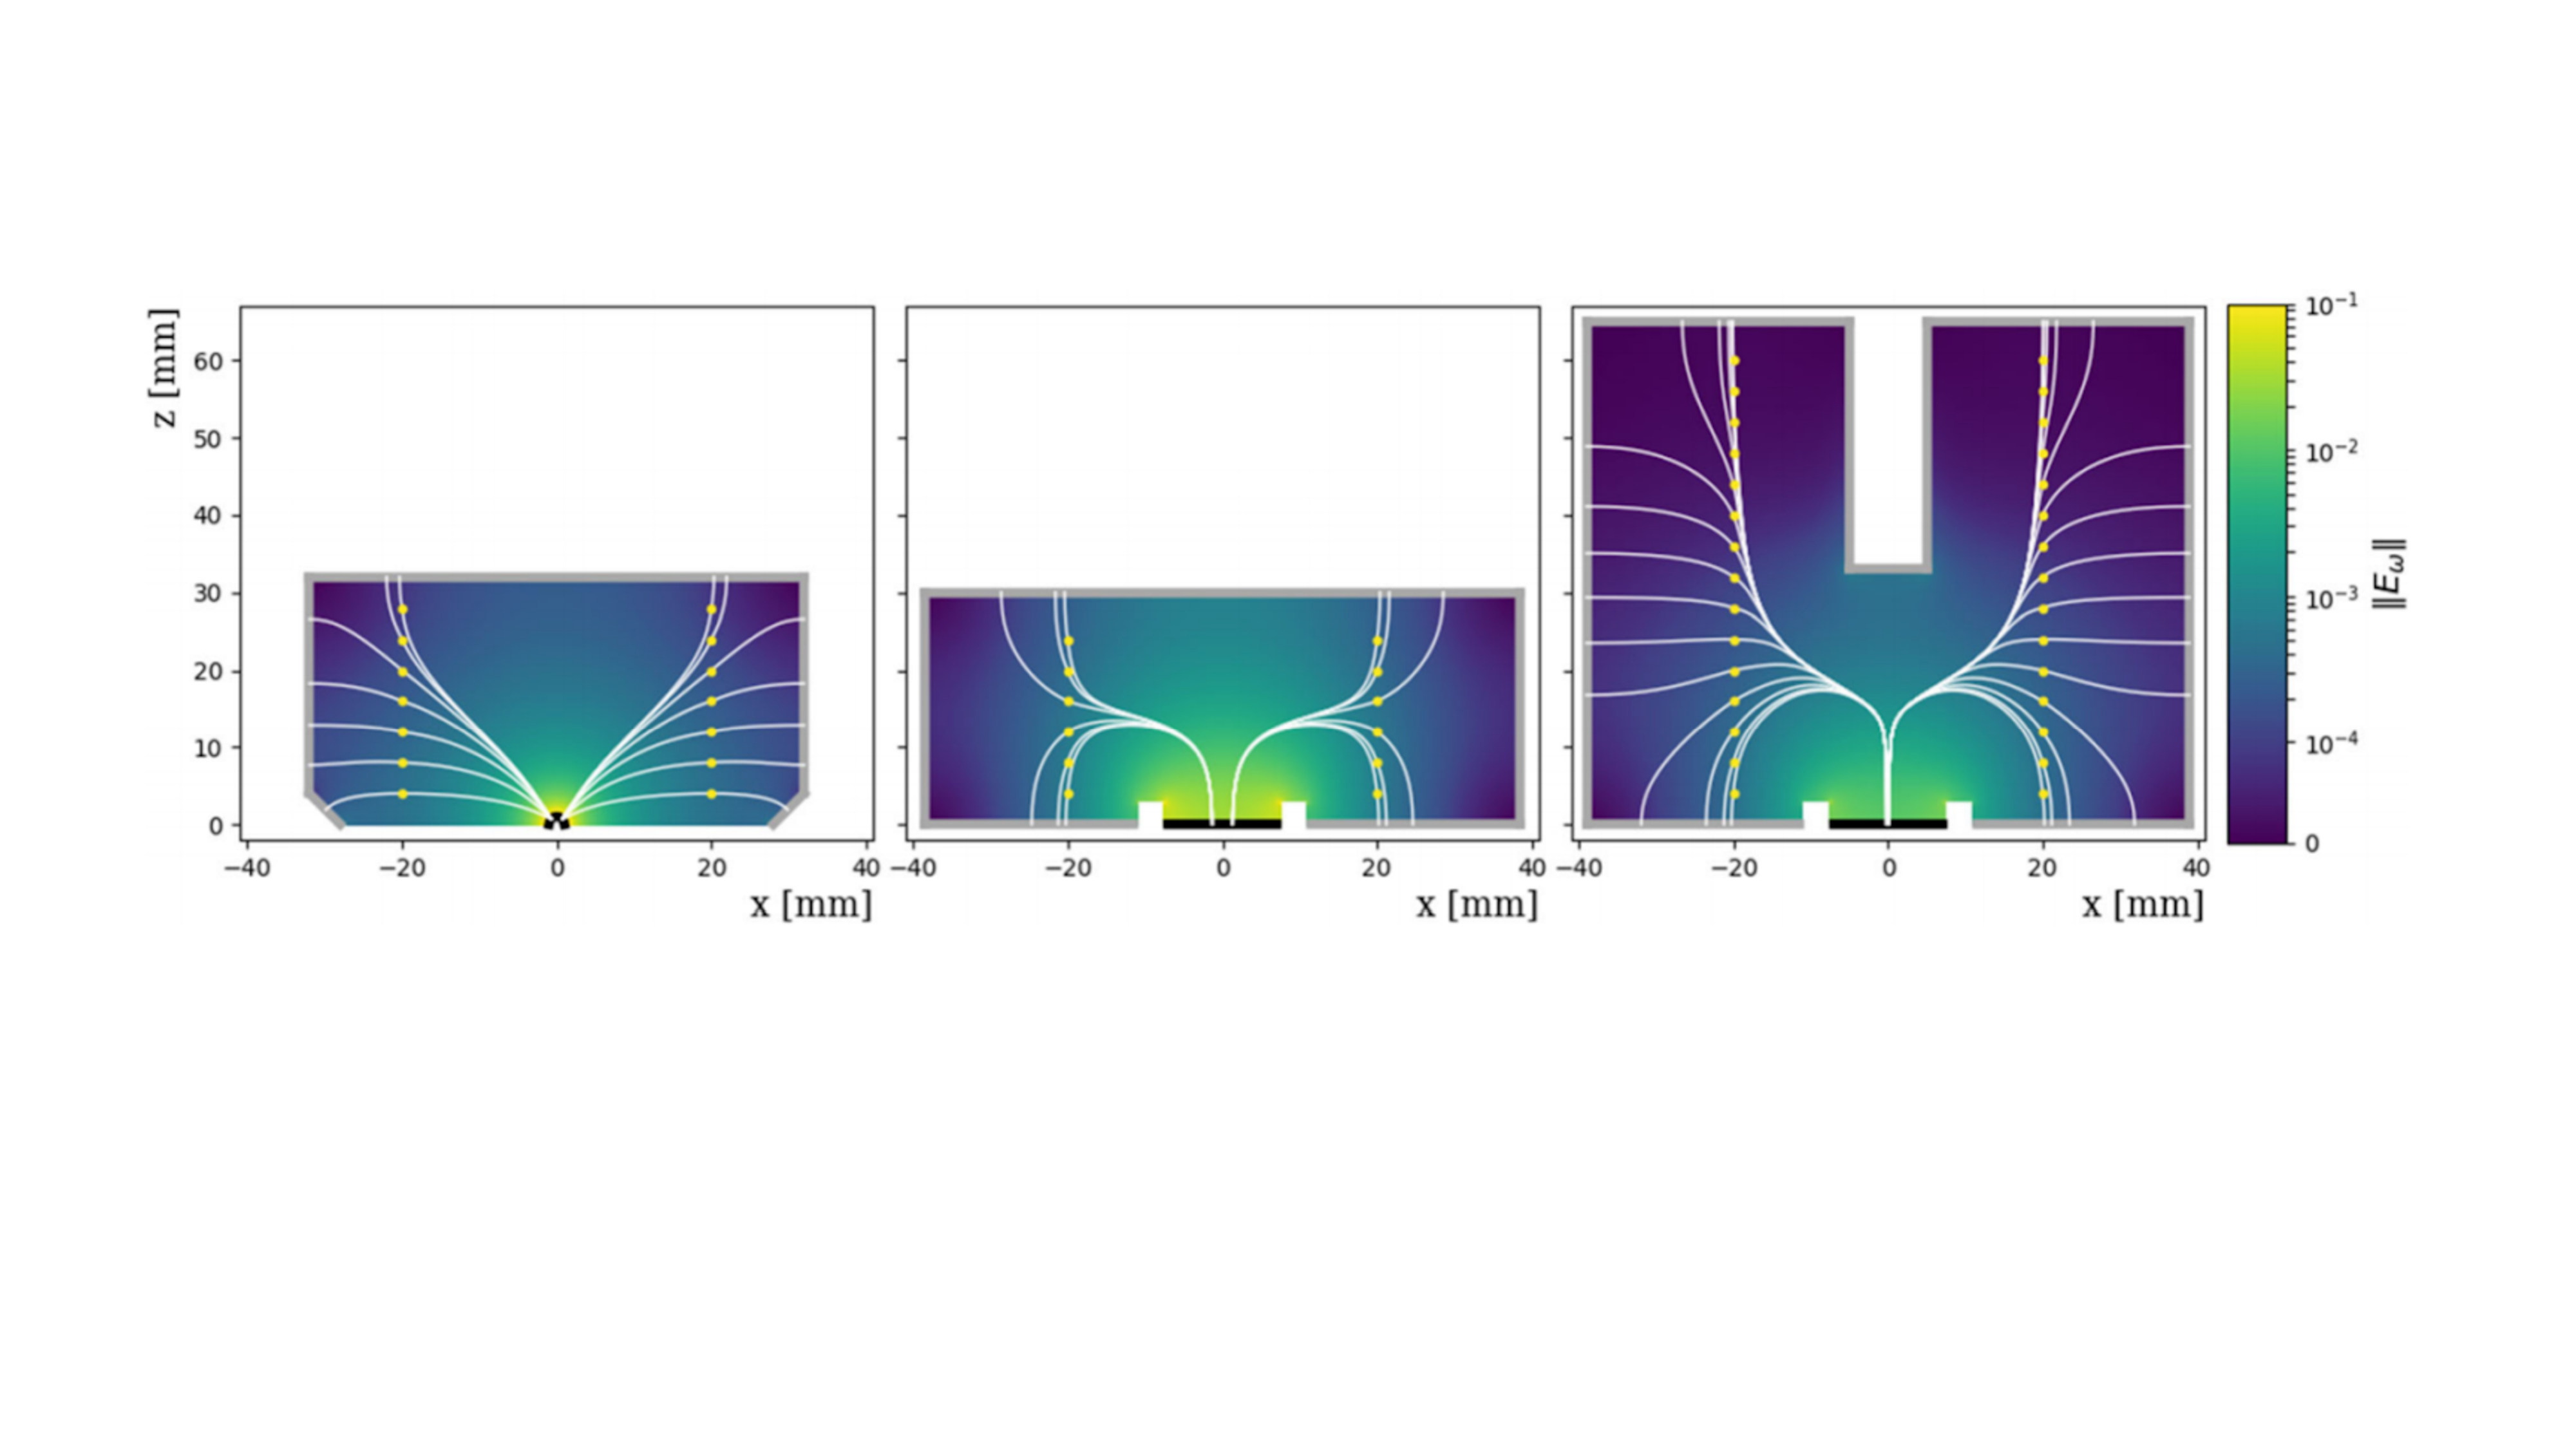
\includegraphics[trim=15 30 15 20,clip,width=\linewidth]{ch2/figs/Det-geo-2.pdf}
\caption{The three point contact detector geometries used in LEGEND: {\MJD} PPC detectors (left), {\Gerda} BEGe detectors (middle), and newly developed ICPC detectors (right).The color bar depicts weighting potential within each detector's cross section.The thick black and gray lines are the p$^+$ and n$^+$ electrode, respectively. The yellow points are locations of simulated energy depositions. The holes travel along the white lines to the p$^+$ electrode, while electrons travel along while line to the n$^+$ electrode. Figure from \cite{Comellato:2020ljj}.}
\label{fig:det-compare}
  \end{figure}
  
The three types of point contact detector geometries that LEGEND uses are illustrated in Figure \ref{fig:det-compare}. The p$^+$ contact is created by implantation of boron at the crystal end with the highest impurity. The n$^+$ region is created by diffusion of lithium atoms onto the detector surface. To isolate the two electrodes from each other, the surface region in between is passivated, usually with amorphous germanium. The BeGe and ICPC detectors also have a passivated ditch. The electric field is carefully designed by controlling the geometry and impurity gradient in the crystals. 


{\Ltwo} took physics data in a $142$ kg source configuration from March 2023 until February 2024. The first data set was unblinded on 13 June 2024. After applying analysis cuts, a total of seven events were observed in the region of interest, corresponding to a background index of $ (5.3 \pm 2.2) \times 10^{-4} \text{ cts/(keV$\cdot$kg$\cdot$yr)}$. In a combined fit of {\Gerda}, {\MJD}, and {\Ltwo}, the lower limit on the 0$\nu\beta\beta$ half-life was set at $T^{0\nu}_{1/2} > 1.9 \times 10^{26} \text{ yr} \quad \text{(90\% C.L.)}$ with an expected sensitivity of $2.8 \times 10^{26}$ years. \cite{Pertoldi2024}

\subsection{LEGEND-1000}
The subsequent phase of LEGEND is a proposed ton-scale experiment that will probe the entire inverted ordering mass hierarchy, with the capability to make an unambiguous discovery of {\onbb} with $3\sigma$ certainty for the $m_{\beta\beta}$ range of $9$-$21$ meV. It would also cover half of the normal ordering parameter space, under certain assumptions \cite{l1000_pcdr}. LEGEND-1000 builds on the innovation and research done in {\Ltwo}. It will use only ICPC detectors, which have demonstrated lower surface backgrounds, excellent energy resolution, and precise pulse shape discrimination. The experiment also plans to use underground-sourced liquid Ar, which would greatly reduce the $^{42}$K background. LEGEND-1000 would probe a half-life of $10^{28}$ years after $10$ years of live time. The preconceptual design report for LEGEND-1000, with a detailed design description and information about the discovery potential, can be found at \cite{l1000_pcdr}. {\Ltwo} will be the main scope of this thesis, with the aim of developing techniques for {\Lthou}.


%\subsection{Pulse Shape Discrimination}


\section{{\Ltwo} background model}
{\Ltwo} has very low backgrounds. Figure \ref{fig:L200_background} shows the expected background contribution in {\Ltwo} at $Q_{\beta \beta}$ after all analysis cuts. These contributions were calculated using radiopurity assays of selected materials and Monte Carlo simulations. 

\begin{figure}[!htb]
\centering
  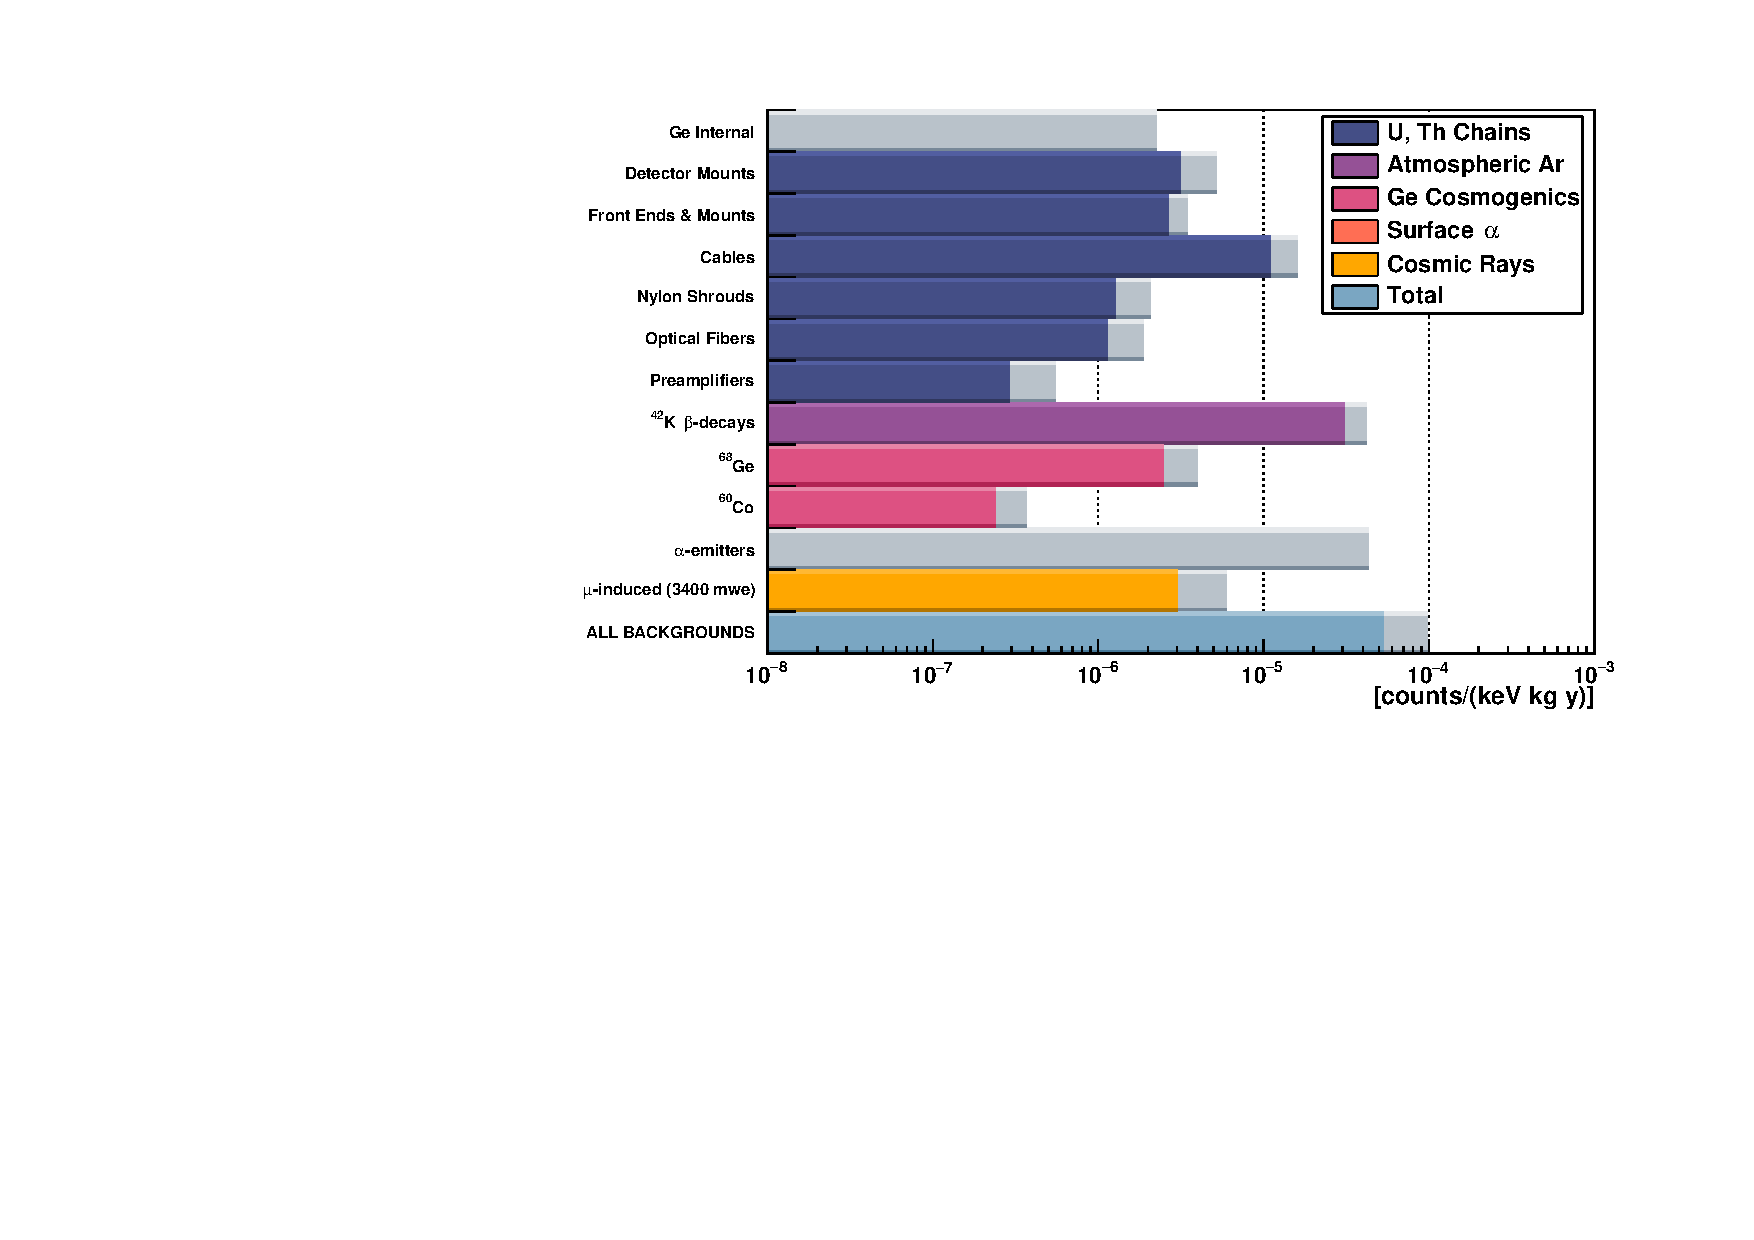
\includegraphics[width=0.99\linewidth]{ch2/figs/L200_background.pdf}
  \caption{{\Ltwo} Projected background contributions near Q$_{\beta\beta}$ after all analysis cuts. Grey bands indicate uncertainties in assays and background rejection.}
\label{fig:L200_background}
  \end{figure}

The decays of long-lived isotopes $^{238}$ U and $^{232}$ Th, as well as their short-lived progeny, are the main backgrounds of component materials. They are primarily reduced by using higher purity materials and by reducing materials near the detectors. 

Cosmogenic backgrounds from $^{68}$Ge and $^{60}$Co isotopes are produced when the HPGe crystal is exposed to neutrons produced by cosmic rays. This background can be reduced by controlling the cosmic-ray exposure during detector production and increasing the underground cool-down period for the HPGe detectors prior to the experiment.

{\onbb} events are inherently single-site. Most background events in HPGE deposit energy in multiple locations. During the analysis, LEGEND approaches these backgrounds using two broad techniques: Pulse shape discrimination (PSD) and Anti-Coincidence (AC) tagging.

The HPGe point contact configuration enables identification of the unique drift of the charge clouds for each location. PSD techniques take advantage of this ability to reject multi-site and surface backgrounds. An example of a PSD technique is the use of the A/E discriminator, which relies on the maximum value of the derivative of the waveform, the current amplitude. Figure \ref{ch2_fig_cur_exp} shows the current amplitude for four different events in the experiment: n$^+$ surface beta event, p$^+$ surface alpha event, a multi-site gamma event and a single-site signal event, such as a {\onbb} or {\tnbb} event. Each event has a unique current signal, and the maximum value of the current provides an effective way to accept or reject them. The cuts are very effective at rejecting backgrounds, but their precise level of effectiveness is difficult to measure, particularly for surface backgrounds, as we do not have access to a large or pure sample of this category of events. Knowing this rejection efficiency helps us improve PSD cuts and is needed to predict background in future experiments, like {\Lthou}.
%For example, the first results of {\Ltwo} indicate the PSD efficiency of $86.4 \pm 3.5 \%$ in the ICPC detectors. \cite{Engelhardt2024}


\begin{figure}[!htb]
\centering
  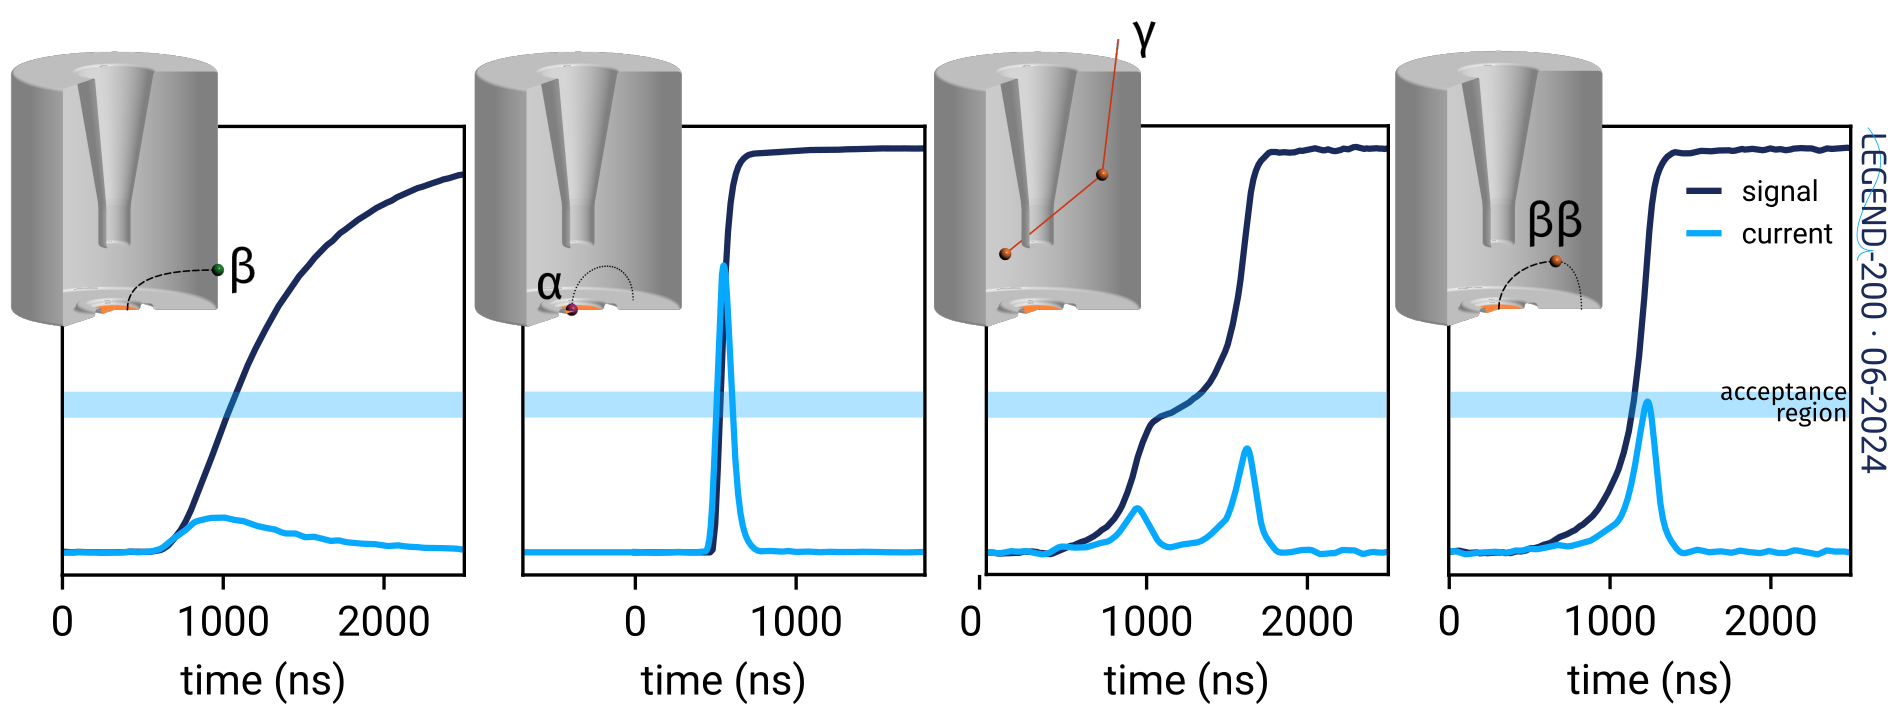
\includegraphics[width=0.99\linewidth]{ch2/figs/psd-showcase.png}
  \caption{Signal (black) and current (blue) for four different types of events in {\Ltwo}. The point contact geometry enables long and unique drift times that allow for pulse shape discrimination. The maximum of the current signal can be used to reject the three background events and accept the {\tnbb} events. Credit: The LEGEND Collaboration.}
\label{ch2_fig_cur_exp}
  \end{figure}
  
The AC cuts are used to detect background depositing energies at multiple locations. The liquid argon cut rejects events that happened in the germanium detector while producing scintillation in the LAr volume. Similarly, the Muon veto rejects events that produce Cherenkov light in the water tank. Finally, the granularity cut removes events producing energy depositions in multiple HPGe detectors.

$^{42}$ K betas are among the largest contributions to the background. These backgrounds come from betas that interact on all surfaces of the detectors. At the n$^+$ surface, the thick dead layer blocks some of the betas from reaching the active volume, but PSD is the most important tool in reducing these backgrounds. The use of liquid Argon introduces two short-lived isotopes, $^{39}$Ar and $^{42}$Ar.  $^{42}$Ar decays into $^{42}$K which is positively charged and can drift with the applied electric field to the detector surface. Then it can undergo a beta decay with a Q value of $3525$ keV that overlaps with the region of interest. $^{42}$Ar is formed by cosmogenic exposure to atmospheric Ar, and the best way to mitigate its background is to use underground-sourced Argon, as proposed for LEGEND-1000. {\Ltwo} uses nylon shrouds that inhibit the drift of $^{42}$ K ions. AC and PSD cuts further help to identify the beta background.

Alpha backgrounds are p$^+$ and passivated surface events that are derived primarily from surface contaminants such as $^{210}$Po and $^{210}$Pb. These originate from the decay of the natural $^{222}$ Rn gas that is adsorbed on the surface during the fabrication, storage, and assembly processes of the detectors. Components can also develop static charges that can increase adsorption. Alpha backgrounds can be reduced by handling the detectors and surrounding materials with care in ultraclean and Rn-reduced environments. In LEGEND, support materials are etched using acids or leached in Nitric acid to reduce the adsorption of radon gas, and then the detectors are assembled and installed into cryostats using a glovebox with a radon-reduced dry Nitrogen environment. The use of liquid Argon reduces the alpha background due to the gaseous $^{222}$ Rn previously observed in MJD. 

\begin{figure}
\centering
  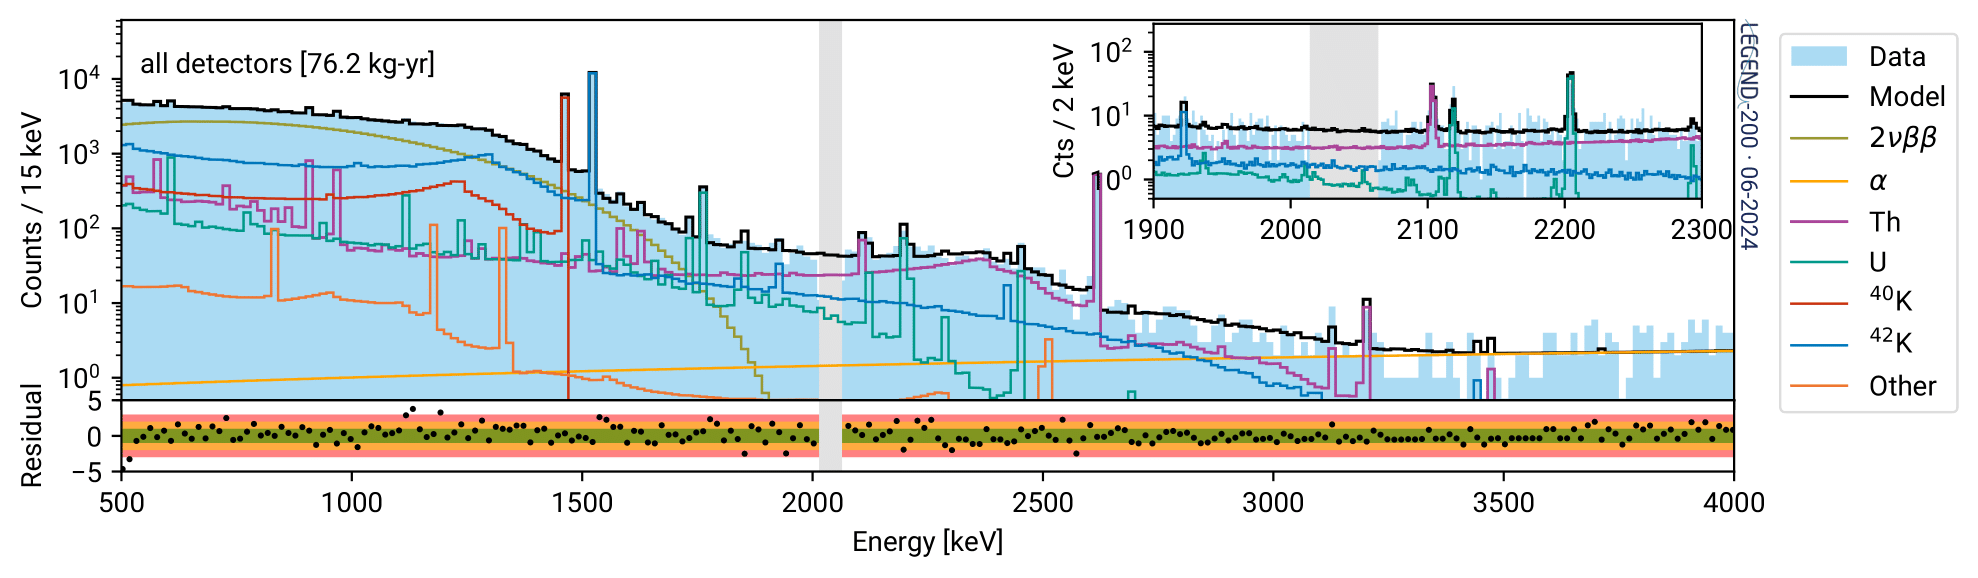
\includegraphics[width=0.99\linewidth]{ch2/figs/l200_bkgmodel.png}
  \caption{{\Ltwo} background contributions near Q$_{\beta\beta}$ after all analysis cuts. Credit: The LEGEND Collaboration.}
\label{ch2:fig:L200_background_model_fit}
  \end{figure}

The alpha background contribution in figure \ref{fig:L200_background} is estimated based on the rate of high-energy background events and their survival after cuts, as observed in GERDA. This is both a small sample size and an extrapolation to the {\onbb} region of interest and, therefore, has a high uncertainty. These uncertainties are driven by uncertainty in the pulse shape rejection for background components in the {\onbb} region of interest. Since there is no first-principles background model for surface events, it is hard to estimate the fraction of background events that leak through the cuts. Passivated surface effects can also affect signal efficiency. If an event occurs near the passivated surface, the surface effects may lead the detector to measure a lower energy than the actual deposited event. Thus, the event might not be registered as {\onbb}, which then reduces the active detector volume for {\onbb} events and distorts the shape of the {\tnbb} spectrum. 

Figure \ref{ch2:fig:L200_background_model_fit} shows the fit of the background model to the data in LEGEND-200. It is constructed using a global binned likelihood fit using measured spectra, radio assay data, and Monte Carlo simulations. The alpha background was modeled using an analytic spectral shape model developed by the {\Gerda} Collaboration. \cite{GERDA_2019cav}. {\Gerda} used multiple PDFs corresponding to different $p^+$ contact thicknesses to model partial energy deposits of alpha decays on the passivated surface. This is combined with a linear continuum to handle highly degraded events. Although the overall background model accurately describes the gamma-induced background, the alpha background component at Q$_{\beta \beta}$ is mostly flat and remains poorly constrained due to modeling challenges. The {\Gerda} model is not effective for {\MJ} PPCs, which have a larger passivated surface.

Pulse Shape Simulations (PSS) model how the charge carriers move and induce signals in the HPGe detectors. PSS enable improved detector design, position reconstruction, and improved pulse shape discrimination by accurately modeling the geometry and electric fields of each detector. They are also key to estimating which background events remain after analysis cuts. Thus, PSS are critical for identifying the sources of background in current experiments and projecting background levels in future searches. Two longstanding obstacles have hindered reliable PSS: incomplete models of charge collection from surface event interactions and the complexity of replicating the detector’s electronic response.

In this work, we focus on methods to improve PSS to model the backgrounds. Chapter 3 focuses on the challenges involved in modeling alpha interactions on the passivated surfaces. The chapter introduces the {\ehd} simulation, which can model surface events using charge diffusion, self-repulsion, and reduced mobility on the surface. Chapter 4 addresses the computational challenges posed by the {\ehd} by showing how the simulation can be accelerated by using GPU computing techniques, enabling large-scale parallelism. Chapter 5 presents the results of {\ehd} simulations. It shows how {\ehd} can reproduce data from test stands, estimate efficiency losses in the region of interest for {\onbb} events, and generate detector-physics-driven spectra for surface backgrounds.

Chapter 6 transitions to the challenge of replicating the detector’s electronic response. It describes how the readout chain modifies waveforms, why first-principles approaches are difficult, and how CPU-Net, a deep learning framework, can improve electronics modeling. Chapter 7 explains the data preparation, simulation pipelines, and training procedures for the neural network–based electronics model. Chapter 8 presents the outcomes of CPU-Net, showing how simulated pulses can be translated into realistic detector-like waveforms and analyzes network performance on critical pulse-shape parameters.
